\documentclass{report}
\usepackage[utf8]{inputenc}
\usepackage{natbib}
\usepackage[pagestyles]{titlesec}
\usepackage{graphicx}
\usepackage{multicol}
\usepackage{multirow}
\usepackage{booktabs}
\usepackage{array}
\newcolumntype{L}[1]{>{\raggedright\arraybackslash}p{#1}}
\newcolumntype{C}[1]{>{\centering\arraybackslash}p{#1}}
\newcolumntype{R}[1]{>{\raggedleft\arraybackslash}p{#1}}


\titleformat{\chapter}[display]{\normalfont\bfseries}{}{0pt}{\Huge}
\newpagestyle{mystyle}
{\sethead[\thepage][][\chaptertitle]{}{}{\thepage}}
\pagestyle{mystyle}

\title{Front Page Test}
\author{AmorosiniCasaliFioravanti}
\date{October 2019}

%TODO: Se non troviamo una copertina migliore prima di consegnare 
%      il progetto eliminiamo la prima pagina e ne facciamo una con paint

\begin{document}
\maketitle 
\tableofcontents
\chapter{Introduction}
This document represents the Requirement Analysis and Specification Document (RASD) for SafeStreets: an application that aims to improve the safety of urban areas by giving its users the possibility to report parking violations and accidents to authorities. The goal of this document is to supply a description of the system in terms of its functional and non functional requirements, listing all of its goals, discussing the constraints and the limits of the software, and indicating the typical use cases that will occur after the release. This document is addressed to the stakeholders, who will evaluate the correctness of the assumptions and decisions contained in it, and to the developers who will have to implement the requirements.
\section{Purpose}
SafeStreets is a crowd-sourced application that intends to provide users with the possibility to notify authorities when traffic violations and accidents occur. In order to report a traffic violation, users have to compile a report containing a picture of the violation, the date, time, position, and type of violation. SafeStreets stores all the information provided by users, completing it with suitable metadata (timestamps, sender's GPS if available, etc.). In particular, in case the user had not provided any information regarding the license plate of the car breaking the traffic rules, SafeStreets runs an algorithm to read it from the submitted picture. Moreover, the application allows both end-users and authorities to mine the information that has been received: this function allows users to perform useful statistics, for example to find out which area is more dangerous or which vehicles commit the most violations. If the municipality offers a service that allows users to retrieve the information about the accidents that occur in its territory, SafeStreets can cross this information with its own data to identify potentially unsafe areas, and suggest possible interventions.
In addition, the municipality could offer a service that takes the information about the violations coming from SafeStreets, and generates traffic tickets from it. In this case, SafeStreets ensures that the chain of custody of information coming from users is never broken, thus information is never altered. Information about issued tickets can be used by SafeStreets to build statistics, for example to have a feedback on the effectiveness of the application.
\subsection{Goals}
\begin{itemize}
    \item {[G.1]} The System allows the Users to access the functionalities of the application from different locations and devices.
    \item {[G.2]} The System allows Guests to authenticate themselves either as Authority or Citizen.
    \begin{itemize}
    		\item {[G.2.1]}The System offers different levels of visibility to different roles.
    \end{itemize}
    \item {[G.3]} The System allows the Citizens to document traffic violations and accidents to Authorities by compiling a Report.
    \item {[G.4]} The System stores the reports provided by the Citizens.
    \begin{itemize}
    		\item {[G.4.1]} If the Citizen has not provided any information about the license plate, the System runs an algorithm to read it from the submitted picture.
    	\end{itemize}     
    %\item {[G.6]} The System allows the Citizens to add testimony of an accident they have seen.
    \item {[G.6]} The System analyzes the stored information to detect unsafe areas.
    \begin{itemize}
    		\item {[G.6.1]}If the System collects multiple reports for the same problem in a given area, it can suggest possible interventions to the Authorities.
    		\item {[G.6.2]}If allowed by Authorities, SafeStreets can cross their information about accidents with its own in order to improve the analysis.
    \end{itemize}    
    \item{[G.7]} If allowed by Authorities, SafeStreets can access their information about issued tickets to build statistics and evaluate its effectiveness.
    \begin{itemize}
        \item {[G.7.1]} The System ensures that the chain of custody of the information coming from the Citizens is never broken.
    \end{itemize}
\end{itemize}

\section{Scope}
% Stuff on world and shared phenomena
According to the \textit{World} and \textit{Machine} paradigm, proposed by M. Jackson and P. Zave in 1995, we can distinguish the \textit{Machine}, that is the portion of the system to be developed, from the \textit{World}, that is the portion of the real-world affected by the machine. In this way, we can classify the phenomena in three different types: World, Machine and \textit{Shared} phenomena, where the latter type of phenomena can be controlled by the world and observed by the machine or controlled by the machine and observed by the world.
\newline
In this context, the most relevant phenomena are organized as in the following table.
\begin{table}[!ht]
		%{pix.acc.} & {mean.acc.} & {mean.IoU} & {f.w.IoU}
		\begin{center}
		%\hspace{-4.5cm}
		\begin{tabular}{|C{3.5cm}||C{3.5cm}||C{3.5cm}|}
			\toprule
			\textbf{World} &\textbf{Shared}& \textbf{Machine}\\
			\midrule
			\textbf{Traffic violation}: circumstance in which someone doesn't respect the traffic rules&\textbf{Registration/Login}$^{1}$: a Guest can sign up to the application or log in if already registered.&\textbf{DBMS query}: operation performed to retrieve/store data\\
			\midrule
			\textbf{Accident}:event that caused damage to things or people.&\textbf{Commit of a report}$^{1}$: action of sending a report documenting a traffic violation or an accident.&\textbf{API queries}: request for third-part services.\\
			\midrule
			&\textbf{Build statistics}$^{2}$: computation of statistics to find unsafe areas, to see which veichles commit multiple infractions and also to monitor the trend of issued tickets.&\textbf{use of Hash}: compute the hash function to ensure that information is never altered.\\
			\midrule
			&\textbf{Safety suggestions}$^{2}$: to give suggestions for possible safe interventions (e.g add a barrier).&\textbf{Credential validation}: checking that Citizens can not access as Authorities\\ 
			\midrule
			%\textbf{Generation of traffic tickets}$^{1}$: to generate traffic tickets using the information about traffic violation.&	\\			
			\midrule
			&\textbf{Send notification}$^{2}$: to notify the Autorithies when a report is submitted.&\\
			\bottomrule
		\end{tabular}
		\end{center}
		\caption{In the table above, \textit{1} refers to shared phenomena controlled by the world and observed by the machine, whereas \textit{2} refers to the phenomena controlled by the machine and observed by the world}
		\label{tab:multicol}
	\end{table}
	
\section{Definitions, Acronyms and Abbreviations}
\subsection{Definitions}
\begin{itemize}
	\item \textit{System}: the totality of the hardware/software applications that contribute to provide the service concerned.
    \item \textit{Guest}: someone who has yet to sign up and who is not able to access any feature of the application.
    \item \textit{User}: a registered user who has logged in.
	\begin{itemize}
		\item \textit{Citizen}: end-user who can send Reports of traffic violation. It has limited visibility over the stored information.
		\item \textit{Authority}: user who has access to the history of Reports and is notified whenever a new Report is recieved. It has full visibility over the data exposed by the System.
	\end{itemize} 
    %\item \textit{Logged in User}: a registered user who logged in.
    \item \textit{Report}: documentation of a traffic violation. It contains a picture of the violation, the date, time, position, and type of violation. Some fields can be omitted in case an accident is being reported.
    \item \textit{Hash}: a mathematical algorithm that maps data of arbitrary size to a bit string of fixed size. It is a one-way function, that is, a function which is practically infeasible to invert.
    \item \textit{Chain of custody}: chronological documentation that records the sequence of custody, control, transfer, analysis, and disposition of physical or electronic evidence.
    \item \textit{Third-party services}: services used by the System in order to provide extra functionalities (e.g. image recognition).
    %\item \textit{Notification}: message that advise the Authorities of a traffic violation.
\end{itemize}
\subsection{Acronyms}
\begin{itemize}
\item \textbf{API}: \textit{Application Program Interface}, set of routines, protocols and tools for building software applications on top of this one.
\item \textbf{OCR}: \textit{Optical Character Recognition}, software dedicated to the detection of characters contained in a document and to their transfer to digital text that can be read by a machine. In this context, OCR will be used to read license plates.
\item \textbf{GPS}: \textit{Global Positioning System}, system widely used to get the user's position.
\item \textbf{DBMS}: \textit{Data Base Management System}, system which provides organized space memory to store information.
\end{itemize}
\subsection{Abbreviations}
\begin{itemize}
\item {[G$_{i}$]}: i-th goal.
\item {[R$_{i}$]}: i-th functional requirement.
\item {[D$_{i}$]}: i-th domain assumption.
\end{itemize}
\subsection{Reference Documents}
\subsection{Document Structure}
The rest of the document is organized as follows:
\begin{itemize}
\item{\textbf{Overall description}}: this section gives a general description of the application, focusing on the context of the system and giving further details about shared phenomena. Furthermore, we will provides the specifications of constraints, dependencies and assumptions, that show how the System is integrated in the real world.
\item{\textbf{Specific requirements}} this section goes into the details about functional and non-functional requirements and a list of all possible interctions with the System is provided using use cases and sequence diagrams.
\end{itemize}

\chapter{Overall Description}
\section{Product Perspective}
We are going to analyze all the shared phenomena that are listed in the previous section. The concepts are clarified throw class and state diagrams.\\
\\
\textbf{Registration/Login} (world controlled, machine observed)\\
A User can sign up to the application or log in, if is already registered. 
In the case of a new submit, the System provides a form which the User have to fill with his data, specifying if he/she is 
a Citizien or an Authority. Then the data are collected in the associated DBMS.\\
\\
\textbf{Commit of a report} (world controlled, machine observed)\\
A User can send a report with a description of the violation compiling a structured field. He/she has the possibility to  attach a picture. The System will check if the informations inserted in the fields are consistent and complete, then will send them to the
DBMS.\\
\\
\textbf{Build statistics} (machine controlled, world observed)\\
The System computes general statistics on the violations, and also finds unsafe areas. These general information can be seen by the Citizens. Other specific statistics are accessible only by Authorities an example is
the vehicles which commits multiple infractions, and also to see how the trends of issued tickets change. \\
\\
\textbf{Safety suggestions} (machine controlled, world observed)\\
The System gives suggestions for possible safe interventions. His knowledge is based on data statistics.\\
\\
%\textbf{Generation of traffic tickets} (machine controlled, world observed)\\
%The Authorities can compile a legal form to make a traffic ticket, using the information about traffic violation. 
%The System provides security tools to protect sensible data.\\
%\\
\textbf{Send Notification} (machine controlled, world observed)\\
The System notifies a logged Authority when a report is submitted by an User. 
Then the Authority takes the right legal measure based on the information that he/she gets.
%Something later
\chapter{Specific Requirements}
%stuff..
\subsection{Class Diagram}
\begin{figure}
\begin{center}

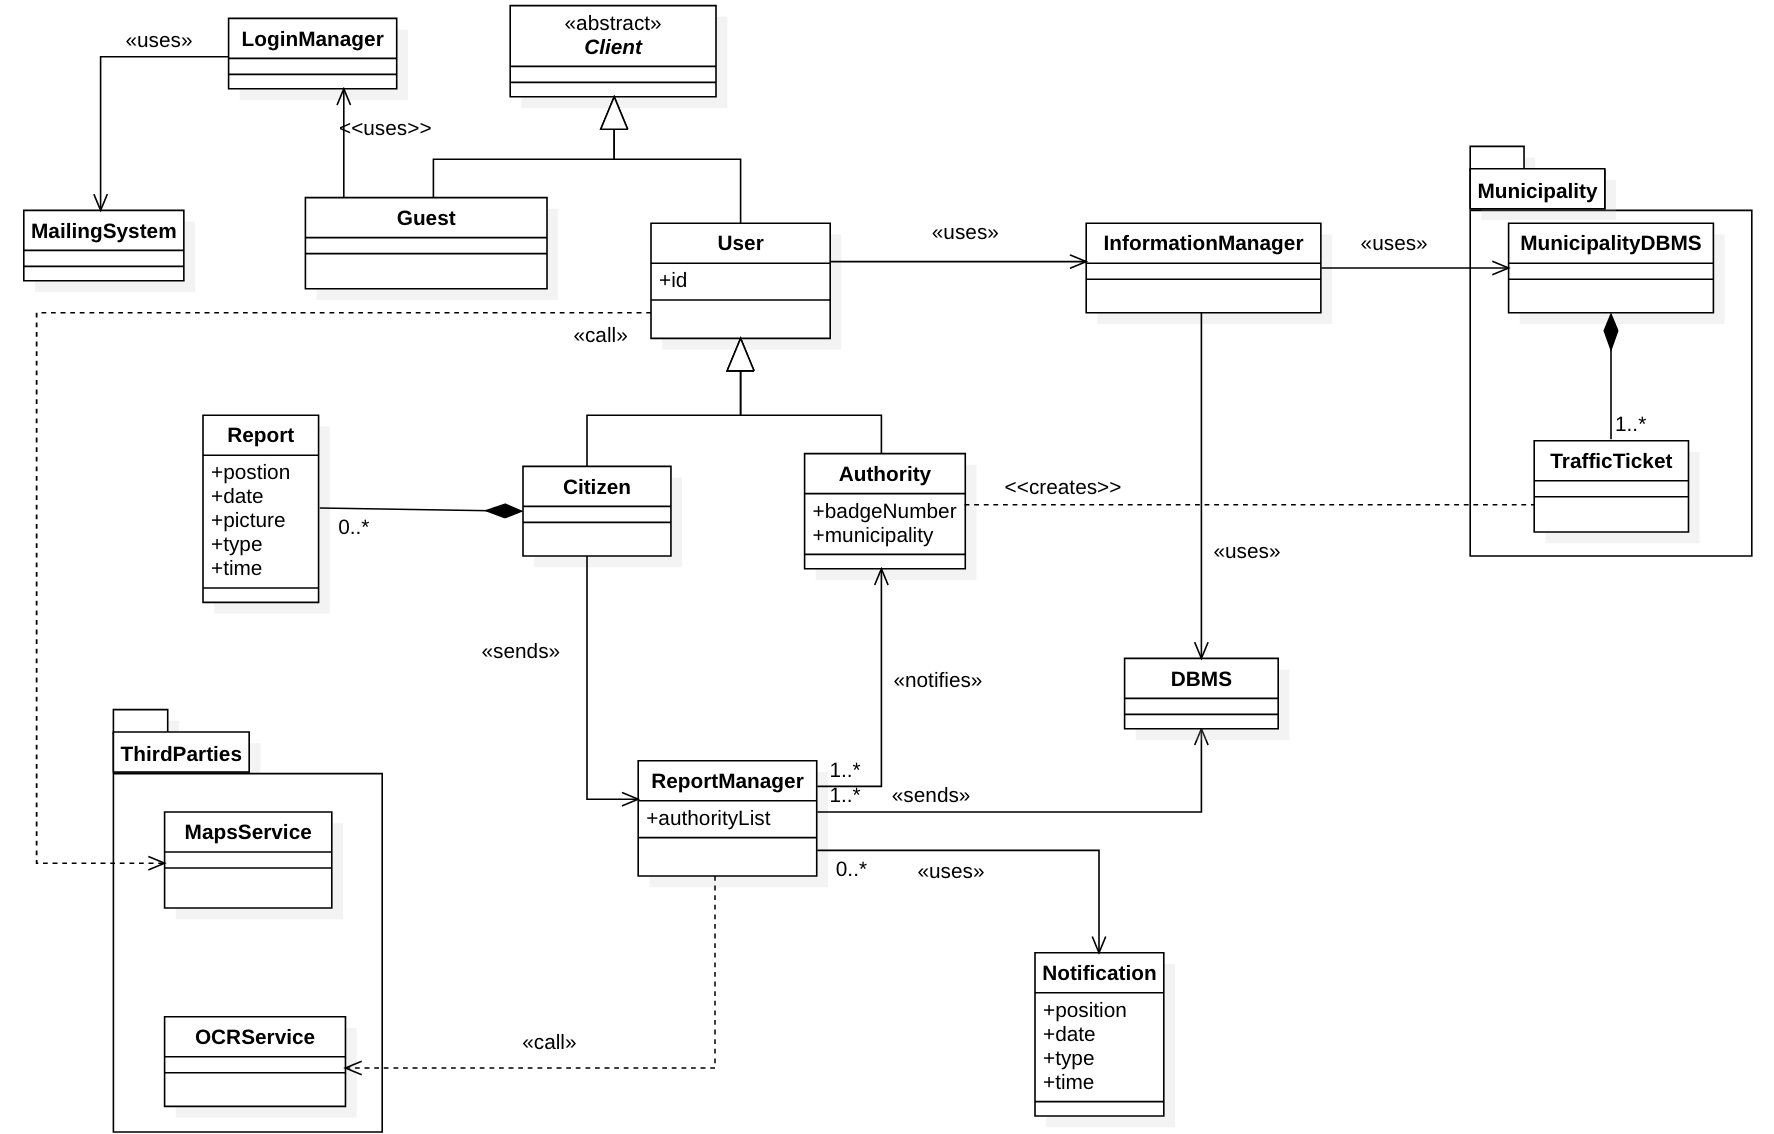
\includegraphics[scale=0.4]{/home/tommaso/Scrivania/img/SWE1.png}
\end{center}
\caption{Schema riassuntivo per la visualizzazione dei passaggi fondamentali.}
\label{schema}
\end{figure} 
\section{Functional Requirements}
%TODO: Requirements
che erano goal, da aggiustare successivamente
\begin{itemize}
\item {[G.4]} The Report Manager handles the submissions:
    {\setlength\itemindent{25pt} \item {[G.4.1]} Before accepting any Report, the Report Manager ensures that it contains a picture of the violation, the date, time, position, and type of violation.}
    {\setlength\itemindent{25pt} \item {[G.4.2]} The Report Manager notifies all logged in Authorities whenever a new Report is accepted.}
    {\setlength\itemindent{25pt} \item {[G.4.3]} The Report Manager must ensure that no more than one Authority has taken in charge the same Report.}
    {\setlength\itemindent{25pt} \item {[G.4.4]} The Report Manager notifies Citizens whenever one of their Reports has been taken in charge by an Authority.}
\item {[G.9]} The System can accedes to the stored traffic tickets with a permission from the local municipality.
\end{itemize}their
\end{document}